\chapter{Design}
\label{Chapter:Design}

\section{System Architecture}
\begin{figure}[H]
  \centering
  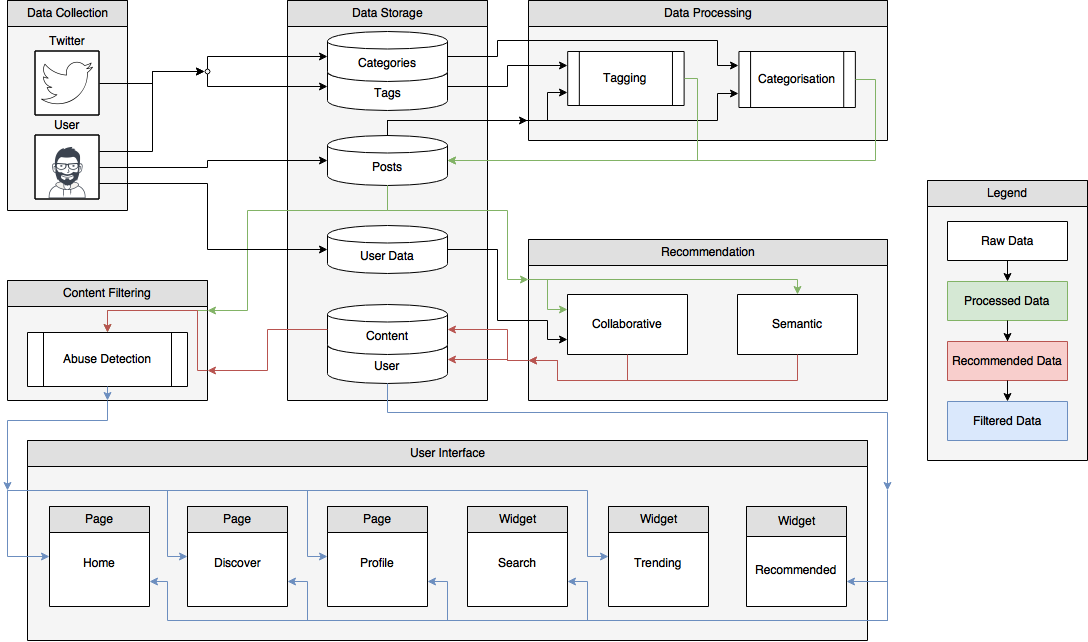
\includegraphics[width=1.0\textwidth]{Images/Design/SystemArchitecture}
  \caption{Proposed System Architecture Diagram} \label{fig:SystemArchitecture} 
\end{figure}

\section{Data Collection}

\section{Data Processing}
\subsection{Abuse Detection}
\subsection{Content Filtering}
\subsection{Recommendations}
Recommendations are a key component to Fidelis, and this section will look at the design of the algorithms for this purpose. Collaborative-based filtering was chosen as the filtering technique for recommendations. JustIfication for this is apparent in the technique itself; collaborative-filtering focuses on using the opinions of like-minded users, coupled with items rated by the user in the past. This sets up recommendations for success as they are much more likely to be greeted positively by the user. Given the nature of Fidelis as social network, resources in terms of previously rated items (through votes on posts) and like-minded users will be available in abundance to generate strong recommendations. It is important to provide the user with choice for how they would like to receive recommendations. To this end, the user will be provided with the option to choose how their recommendations should be provided. The following sections will look at the algorithm that will be used to generate recommendations for users, and will also discuss three different recommendation flavours that will be offered to the user, giving them final say on how their recommendations are generated. The algorithms discussed in the following sections only deal with user recommendations, but the same approaches are applied to generate content recommendations as well.

Users are likely to interact with recommendations they receive on a daily basis. As such, algorithms generating recommendations should run on a daily basis. To generate recommendations, we must therefore first look at the number of recommendations already generated for each user. A user may choose not to interact with provided recommendations, so new recommendations should be made only when a user has approved or rejected their current recommendations. For each user, their item vector should be retrieved. The item vector will correspond to the features discussed in Chapter \ref{Chapter:Research}. The set of candidate recommendations for the user will be determined by what recommendation method they have chosen. In the event that there are no candidate users, a default set of recommendations will be provided for the user. Using the retrieved collection of candidate recommendations, each user in this collection will be assessed to determine whether the similarity between them and the user is sufficiently large. Suitability between users will be determined using a threshold value. We are only interested in similarities that are at least as large as this value, as similarities less than the threshold value would mean that the two users in question are not similar. Only those users with a similarity greater than the threshold value should be provided as a recommendation. Algorithm \ref{alg:recommendations} provides pseudocode for this process. Values for $similarityThreshold$ and $val$ should be set by the user.

\begin{algorithm}
\caption{Recommendations algorithm}
\label{alg:recommendations}
\begin{algorithmic}[1]
\State $similarityThreshold\gets 0.7$
\State $val\gets 5$
\ForAll{users $u$}
	\State $method\gets getRecommendationMethod(u)$
	\State $currentRecommendations\gets getNumberOfRecommendations(u)$
	\If{$currentRecommendations < val$}
		\State $uVector\gets getItemVector(u)$
		\If{$method = Friend$-$of$-$a$-$Friend$}
			\State $users\gets getFOFUsers(u)$
		\EndIf
		\If{$method = Explorer$}
			\State $users\gets getExplorerUsers(u)$
		\EndIf
		\If{$method = Hybrid$}
			\State $fof\gets getFOFUsers(u)$
			\State $explorer\gets getExplorerUsers(u)$
			\State $users\gets fof \cap explorers$
		\EndIf
		
		\State $uFollowing\gets getFollowing(u)$
		\State $users = users \setminus uFollowing$
		
		\If{$\left\vert{users}\right\vert = 0$}
			\State $getDefaultRecommendations$
		\Else
			\For{$v$ in $users$}
				\State $vVector\gets getItemVector(v)$
				\State $similarity\gets measureSimilarity(uVector, vVector)$
			
				\If{$similarity \geq similarityThreshold$}
					\State $storeRecommendation(v)$
				\EndIf
			\EndFor
		\EndIf
	\EndIf
\EndFor
\end{algorithmic}
\end{algorithm}

The following sections will look at each of the possible user sets for candidate recommendations. Each section provides a general overview of the method for user selection and includes a discussion on the method itself with regards to the wider system.

\subsubsection{Friend-of-a-Friend Users}
With this method, candidate recommendations for a user $A$ are all users $C$ where $A$ follows $B$ and $B$ follows $C$. This method uses like-minded users for recommendations, and exploits the transitive nature of the ``following'' relationship. It is a popular technique used by numerous social networks, including Facebook (Figure \ref{fig:fof-facebook}) and Linkedin (Figure \ref{fig:fof-linkedin}).

\begin{figure}[h]
	\centering
	\begin{subfigure}[b]{.3\linewidth}
		
\includegraphics[height=2in]{Images/Design/facebook}
		\caption{}
		\label{fig:fof-facebook}
	\end{subfigure}
	\begin{subfigure}[b]{.5\linewidth}
		
\includegraphics[width=1\linewidth]{Images/Design/linkedin}
		\caption{}
		\label{fig:fof-linkedin}
	\end{subfigure}
	\caption{Friend-of-a-Friend recommendations from (a) Facebook and (b) Twitter}
	\label{fig:fof}
\end{figure}

This option will allow the user to generate ``safer'' recommendations by using the idea that ``if $A$ trusts $B$, and $B$ trusts $C$, $A$ will most likely also trust $C$''. This is not always the case, but mostly holds true. It is important to give users this choice as it provides them more control over who enters their trust circle. Although one of the project aims is to burst opinion bubbles through exposure to different and trusted views, users must still be provided with this option. The function in Algorithm \ref{alg:fof-users} provides a procedure for retrieving ``$C$'' users. 

\begin{algorithm}
\caption{Function for getting Friend-of-a-Friend users}
\label{alg:fof-users}
\begin{algorithmic}[1]
\Function{getFOFUsers}{User u}
	\State $users = \emptyset$
	\State $uFollowing\gets getFollowing(u)$
	\For{$f in uFollowing$}
		\State $fFollowing\gets getFollowing(f)$
		\State Add $fFollowing$ to $users$
	\EndFor
	\State \Return{$users$}		
\EndFunction
\end{algorithmic}
\end{algorithm}

\subsubsection{Explorer Users}
Fidelis aims to expose users to opinions and users they may not necessarily... 
Candidate recommendations are found by finding users' favourite tags to post in and looking at other users who post in the same tag. This user collection method combines the users rated items and looks at like-minded users. By deviating from the users trust circle, we are more likely to generate recommendations that will broaden user opinions by finding other users who care about the same topics, but will naturally hold different views on them. This method seeks to expand a users trust circle beyond current opinions held by them. The function in Algorithm \ref{alg:explorer-users} shows the procedure for collecting Explorer users. $N$ is used to determine the number of tags that will be searched for candidate recommendations. The function in Algorithm \ref{alg:explorer-users} shows this procedure.

\begin{algorithm}
\caption{Function for getting Explorer users}
\label{alg:explorer-users}
\begin{algorithmic}[1]
\Function{getExplorerUsers}{User u}
	\State $threshold\gets 75$
	\State $users\gets \emptyset$
	\State Get $N$ top tags $u$ posts in
	\For{$tag t = 1$ to $N$}
		\State Get all users $v$ posting in $t$
		\If{$reputationOf(v) >= threshold$}
			\State Add $v$ to $users$
		\EndIf
	\EndFor
	\State \Return{$users$}
\EndFunction
\end{algorithmic}
\end{algorithm}

\subsubsection{Hybrid Users}
Using this method aims to find the middle ground between the two aforementioned techniques. The difference between Explorer and Friend-of-a-Friend users is returned as the set of candidate recommendations. 

\begin{figure}
\centering
\begin{tikzpicture}[
    thick]
    \draw [fill=cyan, fill opacity=0.5, name path=c1] (0,0) circle (2cm);
    \draw [fill=orange, fill opacity=0.5, name path=c2] (3,-1) circle (2.5cm);
    \draw (0,0) ++(120:2cm) -- ++(120:2.2cm) node [fill=white,inner sep=5pt](a){Friend-of-a-Friend};
    \draw (3, -1) ++(30:2.5cm) -- ++(30:2.6cm) node [fill=white,inner sep=5pt](b){Explorer};
    \path [name intersections={of=c1 and c2,by=cs}];
    \draw (cs) -- ++(.5,1) node [fill=white,inner sep=5pt](c){Hybrid};
\end{tikzpicture}
\caption{Hybrid user selection}
\label{fig:hybrid}
\end{figure}


\subsubsection{Default Recommendations}
If all aforementioned methods fail to return a set of candidate recommendations, the system should revert to default candidate recommendations. This method will return either the $N$ most popular or reputable users on Fidelis. The function in Algorithm \ref{alg:default-users} shows this procedure for most popular users, but the same procedure can be re-used for getting the most reputable users.

\begin{algorithm}
\caption{Function for getting default users}
\label{alg:default-users}
\begin{algorithmic}[1]
\Function{getDefaultUsers}{User u}
	\State $users\gets \emptyset$
	\State $users\gets getMostPopularUsers$
	\State $users\gets sortDescending(users)$
	\State \Return{$N$ top users from $users$}
\EndFunction
\end{algorithmic}
\end{algorithm}

\subsection{Reputation Scoring}

\section{Database}

\section{User Interface}

\section{Responsive Design}